\documentclass[xcolor=table,mathserif,9pt]{beamer}    % ,handout
% colortbl only defines \rowcolor for a single row. xcolor extends this to multiple rows.

\usetheme{Aachen}
\usepackage[english]{babel}
\usepackage[utf8]{inputenc}
%\usepackage{tikz-dependency}
%\usepackage{chronology}
\usepackage{array, booktabs}
\newcommand{\foo}{\makebox[0pt]{\textbullet}\hskip+0.5pt\vrule width 5pt\hspace{\labelsep}}
\usepackage{multirow}
\usepackage{textcomp}
\usepackage{csquotes}
\usepackage{amsmath}
\usepackage{lipsum}
\usepackage{multicol}
\setlength{\columnsep}{1cm}
%%%%%%%%%%%%%%%%%%%%%%%%%%%%%%%%%%%%%%%%%%%%%%%%%%%%%%%%%%%%%%%%%%%%%%
% tables
\usepackage{multirow,array,tabularx,rotating}
\usepackage{booktabs}
\usepackage{tabularx}

% math
\usepackage{amsmath,amsthm, amssymb, latexsym, xspace}
%\usepackage{bbold}
\usefonttheme[onlymath]{serif}
\boldmath


% misc
\usepackage{subfigure}
\usepackage{wasysym}
\usepackage{nameref}
\usepackage{xcolor}
\usepackage{romannum}
% declare the path(s) where your graphic files are
\graphicspath{{./nlu/}{./g2p/}{./smt/}}
% and their extensions so you won't have to specify these with
% every instance of \includegraphics
\DeclareGraphicsExtensions{.pdf,.jpeg,.png}


%figures
\usepackage{tikz}
\usepackage{minibox}
% change the graphic extentions
%\usepackage{ifpdf}
%\ifpdf
%  \DeclareGraphicsExtensions{.pdf,.png,.jpg}
%\else
%  \DeclareGraphicsExtensions{.eps}
%\fi

\usepackage[np,autolanguage]{numprint}
\nprounddigits{1}

% helpers
\newcommand{\argmin}{\operatornamewithlimits{argmin}}
\newcommand{\argmax}{\operatornamewithlimits{argmax}}
\newcommand{\sign}{\operatornamewithlimits{sign}}
\newcommand{\Eqn}{Equation}
\newcommand{\Eqns}{Equations}
\newcommand{\Fig}{Figure}
\newcommand{\Figs}{Figures}
\newcommand{\Tab}{Table}
\newcommand{\Sec}{Section}
\def\example{{\textit{}{e.g.}}\xspace}
\def\cad{{\textit{}{i.e.}}\xspace}
\def\etc{{\textit{etc.}}\xspace}
\def\apriori{{\textit{a priori}}\xspace}

\newcommand{\NetTalk}{NETtalk\xspace}
\newcommand{\Celex}{Celex\xspace}
\newcommand{\Pronlex}{Pronlex\xspace}
\newcommand{\gtp}{G2P}
\newcommand{\Seg}{\mathbb{S}}
\newcommand\BLEU{\textsc{Bleu}\xspace}
\newcommand\TER{\textsc{Ter}\xspace}
\newcommand\CTER{\textsc{CTer}\xspace}

\newcommand\AER{\textsc{Aer}\xspace}
\newcommand\SAER{\textsc{Saer}\xspace}
\newcommand{\GIZA}{{GIZA\nolinebreak[4]\hspace{-.025em}\raisebox{.2ex}{\small\bf++}}\xspace}

\newcommand{\todo}[1]{\colorbox{yellow}{#1}\xspace}
\newcommand{\CITE}{\colorbox{yellow}{CITE}\xspace}
\newcommand{\REF}{\colorbox{yellow}{REF}\xspace}
\newcommand{\EQ}{\colorbox{yellow}{REF}\xspace}
\newcommand{\NUMBER}{\colorbox{yellow}{NUMBER}\xspace}
\newcommand{\Align}{\mathbb{A}}
%\renewcommand{\emph}[1]{\textcolor{i6blue}{#1}}


\newcommand{\aind}[1]{\hspace*{#1ex}}
\newcommand{\gray}[1]{\textcolor{gray}{#1}}

\newcommand*{\sumw}{\ensuremath{\operatornamewithlimits{sum}}\xspace}
\newcommand*{\nbest}{\ensuremath{\operatornamewithlimits{nbest}}\xspace}

% Define box and box title style
\usepackage{tikz}
\usetikzlibrary{shapes,positioning,fit}
\tikzstyle{bubble} = [ draw=blue, rectangle, rounded corners, inner sep=3pt, inner ysep=
10 pt]
\tikzstyle{fancytitle} =[fill=white, text=black]
\newenvironment{bubble}[3]{%
  \begin{tikzpicture}[transform shape, baseline=-0.5 cm]
  \def\bubbletitle{#1}%
  \node [bubble] (box)\bgroup
  \begin{minipage}[t][#3]{#2}%
}{%
  \end{minipage}%
  \egroup;
  \node[fancytitle] at (box.north) {\bubbletitle};
  \end{tikzpicture}%
}

\newenvironment{bubble*}[2]{%
  \begin{tikzpicture}[transform shape]
  \node [bubble] (box)\bgroup
  \begin{minipage}[t][#2]{#1}%
}{%
  \end{minipage}%
  \egroup;
  \end{tikzpicture}%
}

% CUSTOM STUFF %%%%%%%%%%%%%%%%%
%\usepackage{neuralnetworks}


% Rounding commands
\def\roundpositionii{1}
\newcommand{\rdmii}[1]{\edef\rounded{0}\FPeval\rounded{round(#1,\roundpositionii)}\rounded}
\def\roundpositioni{1}
\newcommand{\rdmi}[1]{\edef\rounded{0}\FPeval\rounded{round(#1,\roundpositioni)}\rounded}
\def\roundposition{0}
\newcommand{\rdm}[1]{\edef\rounded{0}\FPeval\rounded{round(#1,\roundposition)}\rounded}

\npstyleenglish

\def\roundposition{1}
\def\roundpositiont{3}
\edef\rounded{0}
\newcommand{\rd}[1]{\ifthenelse{\equal{#1}{--}}{--}{\edef\rounded{0}\FPeval\rounded{round(#1,\roundposition)}\rounded}}
\newcommand{\rdmt}[1]{\edef\rounded{0}\FPeval\rounded{round(#1,\roundpositiont)}\rounded}
\newcommand{\rp}[1]{%
  \FPset{\per}{#1}%
  %\FPmul{\per}{\per}{100}%
  \FPround{\per}{\per}{1}%
  \numprint{\per}%
}%


\setbeamercovered{transparent}

\DeclareMathOperator*{\sigmoid}{sigmoid}

\newcommand\T{\rule{0pt}{2.2ex}}       % Top strut
\usepackage{etoolbox}
\pretocmd{\section}{\addtocontents{toc}{\vspace{-20pt}}}{}{}

%Table stuff
\newcommand{\tablesize}{}
\newcommand{\abovetable}{\vspace{0.6cm}}
\newcommand{\belowtable}{\vspace{0.13cm}}


% Get fond size for system combination picture right
\usepackage{fix-cm}    
\makeatletter
\newcommand\SyscomFontSize{\@setfontsize\small{6}{60}}
\makeatother   

%%%%%%%%%%%%%%%%%%%%%%%%%%%%%%%%%

\newcommand{\backupbegin}{
   \newcounter{finalframe}
   \setcounter{finalframe}{\value{framenumber}}
}
\newcommand{\backupend}{
   \setcounter{framenumber}{\value{finalframe}}
}

\newcommand{\stoptocwriting}{%
  \addtocontents{toc}{\protect\setcounter{tocdepth}{-5}}}
\newcommand{\resumetocwriting}{%
  \addtocontents{toc}{\protect\setcounter{tocdepth}{2}}}

%%%%%%%%%%%%%%%%%%%%%%%%%%%%%%%%%%%%%%%%%%%%%%%%%%%%%%%%%%%%%%%%%%%%%%  
%%%%%%%%%%%%%%%%%%%%%%%%%%%%%%%%%%%%%%%%%%%%%%%%%%%%%%%%%%%%%%%%%%%%%%

\renewcommand*{\email}{\url{<surname>@i6.informatik.rwth-aachen.de}}  
% all email address(es) of the authors (used for \TitlePage)

\title[NMT]{Neural Machine Translation}
%\subtitle{Presentation Subtitle} % (optional)
%\setbeamertemplate{section in toc}[sections numbered] 
%\setbeamertemplate{subsection in toc}[subsections numbered] 
\setbeamertemplate{navigation symbols}{} %disable {, dotted}navigation bar

%% author and in []: shortauthorChange the scale of beamer from 3.5 to 1
\author[M. Mustermann]{Max Mustermann, and Hermann Ney}
% - Use the \inst{?} command only if the author7s have different
%   affiliation.
\institute[RWTH Aachen University] % (optional, but mostly needed)
{
%  \inst{1}%
  \strut Human Language Technology and Pattern Recognition\\
  \strut Computer Science Department, RWTH Aachen University %\\
  %\strut {\tt lehnen@cs.rwth-aachen.de}
}
% - Use the \inst command only if there are several affiliations.
% - Keep it simple, no one is interested in your street address.

%\date[10/02/2017]{February 10th, 2017}
\date[4/1/2017]{April 1st, 2017}

%%%%%%%%%%%%%%%%%%%%%%%%%%%%%%%%%%%%%%%%%%%%%%%%%%%%%%%%%%%%%%%%%%%%%%shit
% will be set into the PDF document summary
\hypersetup{
  pdftitle={\inserttitle}, 
  pdfauthor={\insertauthor}, 
  bookmarksdepth=subsubsection,  
  % enable automatic page transitions: for endless loop edit in
  % acrobat reader -> preferences -> full screen -> after every X
  % seconds and after last page
  %pdfpageduration = 2, 
  % pdfpagetransition = {Glitter /Di 315 /D 5}  
  % pdfpagetransition = {Box /M /O /D 1},
} 
%%%%%%%%%%%%%%%%%%%%%%%%%%%%%%%%%%%%%%%%%%%%%%%%%%%%%%%%%%%%%%%%%%%%%%
%%%%%%%%%%%%%%%%%%%%%%%%%%%%%%%%%%%%%%%%%%%%%%%%%%%%%%%%%%%%%%%%%%%%%%

%%%%%%%%%%%%%%%%%%%%%%%%%%%%%%%%%%%%%%%%%%%%%%%%%%%%%%%%%%%%%%%%%%%%%%
%%%%%%%%%%%%%%%%%%%%%%%%%%%%%%%%%%%%%%%%%%%%%%%%%%%%%%%%%%%%%%%%%%%%%%
\begin{document}

%%%%%%%%%%%%%%%%%%%%%%%%%%%%%%%%%%%%%%%%%%%%%%%%%%%%%%%%%%%%%%%%%%%%%%
\begin{frame}[label=titlepage]
  \titlepage
\end{frame}

\begin{frame}
	\frametitle{Outline}
	\tableofcontents
        %\tableofcontents[currentsection, subsectionstyle=show/show/hide]
\end{frame}


%%%%%%%%%%%%%%%%%%%%%%%%%%%%%%%%%%%%%%%%%%%%%%%%%%%%%%%%%%%%%%%%%%%%%%

\section{NMT History}
\begin{frame}{NMT History}

\vspace{-1cm}

\begin{table}
\begin{tabular}{@{\,}r <{\hskip 2pt} !{\foo} >{\raggedright\arraybackslash}p{20cm}}
\addlinespace[1.5cm]
2014 & Sequence to sequence translation \cite{NIPS2014_5346, cho-EtAl:2014:EMNLP2014}\\ [8pt]
2015 & Attention-based neural machine translation \cite{BahdanauCB14,Luong-effective}\\ [8pt]
%     & Large Vocabulary NMT \cite{jean}\\ [8pt]
%     & Image caption - NMT \cite{}\\ [8pt]
     
2016 & Subword-NMT \cite{Sennrich2016:bpe}\\ [8pt]

     & Multi-lingual NMT \cite{firat2016multi}\\ [8pt]
%	 & Char-level decoder NMT \cite{char_decoder}\\ [8pt]
%	 & Back-translation NMT\\ [8pt]
	 & WMT 2016\\ [8pt]	 
	 & Google NMT \cite{google_nmt} \\ [8pt]	 
	 & Fully char-level NMT \cite{fully_char_nmt}  \\ [8pt]
2017 & ...
\end{tabular}
\end{table}

\vfill

\end{frame}

%%%%%%%%%%%%%%%%%%%%%%%%%%%%%%%%%%%%%%%%%%%%%%%%%%%%%%%%%%%%%%%%%%%%%%

\section{Sequence to Sequence Translation}
\begin{frame}{Sequence to Sequence Translation }
%\cite{NIPS2014_5346, DBLP:journals/corr/ChoMBB14}}

\begin{itemize}
\item Basic principle behind neural machine translation
\item Translation from one language to another can be done by \textcolor{blue} {a single neural network}
\item The input and output are both variable-length sequences
%\item Probability distribution over all possible translations
\item An encoder reads the source sentence, encodes it into a vector
\item Decoder uses this vector to predict the target words
\end{itemize}

\vspace{1cm}
\centerline{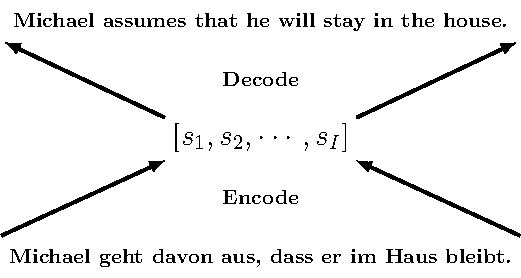
\includegraphics[width=13.0cm]{figures/enc_dec_general}}

\vfill

\end{frame}

%%%%%%%%%%%%%%%%%%%%%%%%%%%%%%%%%%%%%%%%%%%%%%%%%%%%%%%%%%%%

\section{Comparison}

\begin{frame}{Comparison to Best Systems}
\vspace{20mm}
\resizebox{\linewidth}{!}{
  \begin{tabular}{|l|c|c|c|c|c|c|}
  \hline
 & \multicolumn{2}{c|}{WMT2015 De$\rightarrow$En} & \multicolumn{2}{c|}{WMT2016 En$\rightarrow$Ro} & \multicolumn{2}{c|}{BOLT Zh$\rightarrow$En} \\
 & \multicolumn{2}{c|}{newstest2014}              & \multicolumn{2}{c|}{newstest2016}              & \multicolumn{2}{c|}{test1} \\
  \hline
                     & \BLEU\% & \TER\% & \BLEU\% & \TER\% & \BLEU\% & \TER\% \\
\hline
Model A & 28.1    & 53.2   & 24.5    & 59.3   & 17.9    & 67.7\\
Model B & 24.0    & 57.2   & 26.7    & 56.6   & 17.9    & 67.2 \\
Model C & 28.2    & 53.0   & 25.3    & 58.4   & 17.6    & 68.9 \\
\hline
Model D & 29.2    & 52.9   & 27.1    & 55.4   & 21.7    & 63.7 \\
\hline
  \end{tabular}
}

\vspace{20mm}

\begin{itemize}
 \item De$\rightarrow$En and Zh$\rightarrow$En:
 \begin{itemize}
   \item Subwords and LSTM
 \end{itemize}
\end{itemize}

\end{frame}

%%%%%%%%%%%%%%%%%%%%%%%%%%%%%%%%%%%%%%%%%%%%%%%%%%%%%%%%%%%%%%%%%%%%%%%%%%%%%%%%

\begin{frame}[label=finalSlide]
  \label{LastPage}%
  \begin{center}
    \vfill
    {\Large
    \textcolor{i6bluedark}{Thank you for your attention}
    }
%     \vfill
%     \inserttitle
    \vfill
    {\insertauthor}

    \vspace{10mm}
    \url{<surname>@cs.rwth-aachen.de}
  \end{center}
\end{frame}

\nocite{*}

\stoptocwriting
\section{Appendix}
\resumetocwriting

%\backupbegin


%%%%%%%%%%%%%%%%%%%%%%%%%%%%%%%%%%%%%%%%%%%%%%%%%%%%%%%%%%%%%%%%%%%%%%%%%%%%%%%%
\section*{Appendix}

\begin{frame}
  \frametitle{Results: Cool Method with Overlay \only<2>{(WMT2016)} \only<1>{(IWSLT2013)}}
  \only<1>{
  \begin{center}
	\scalebox{0.9}{
\begin{tabular}{|l|cc|cc|cc|cc|}
    \hline
    IWSLT De-En & \multicolumn{2}{c|}{dev} & \multicolumn{2}{c|}{test} & \multicolumn{2}{c|}{eval11} &  \multicolumn{2}{c|}{alignment-test}\\             \hline
    Model & \BLEU\% & \TER\% & \BLEU\% & \TER\% & \BLEU\% & \TER\% & AER\% & SAER\%\\    
    \hline
    Attention-Based & 30.5 & 48.7 & 29.3 & 50.6 & 33.9 & 46.6 & 41.8  & 66.3 \\
     \hspace{3mm}+ method & \textcolor{i6bluedark}{31.5} & \textcolor{i6bluedark}{47.2} & \textcolor{i6bluedark}{30.3} & \textcolor{i6bluedark}{49.0} & \textcolor{i6bluedark}{34.3} & \textcolor{i6bluedark}{44.3} & \textcolor{i6bluedark}{35.4} & \textcolor{i6bluedark}{44.2} \\
    \hline
\end{tabular}
}
	\end{center}}
	\only<2>{
	\begin{center}
\scalebox{0.9}{
\begin{tabular}{|l|cc|cc|cc|}
    \hline
    WMT En-Ro & \multicolumn{2}{c|}{newsdev2016/1} & \multicolumn{2}{c|}{newsdev2016/2} & \multicolumn{2}{c|}{newstest2016} \\             \hline
    Model & \BLEU\% & \TER\% & \BLEU\% & \TER\% & \BLEU\% & \TER\% \\    
    \hline
    Attention-Based & 19.8 & 62.0 & 21.3 & 58.1 & 20.3 & 60.4 \\ 
    +GA & \textcolor{i6bluedark}{21.0} & \textcolor{i6bluedark}{61.1 } & \textcolor{i6bluedark}{23.6} & \textcolor{i6bluedark}{56.4} & \textcolor{i6bluedark}{21.8} & \textcolor{i6bluedark}{59.4} \\ 
    \hline 
    \hspace{3mm} +method + conv ($D=10$,$M=1$) & \textcolor{i6bluedark}{21.4} & \textcolor{i6bluedark}{60.1 } & \textcolor{i6bluedark}{24.7} & \textcolor{i6bluedark}{55.4} & \textcolor{i6bluedark}{22.3} & \textcolor{i6bluedark}{58.7} \\ 
    \hline 
\end{tabular}
}
	\end{center}}
	\vfill
	\begin{itemize}
	  \item Improves translation by an average of $0.8$ BLEU on IWSLT2013
	  \item Great improvement in AER and SAER
	  \item<only@2> Improves translation by an average of $1.7$ BLEU on WMT2016
	  \begin{itemize}
	    \item<only@2> Adding convolutional feedback gives an additional $0.6$ BLEU on average
	  \end{itemize}
	\end{itemize}
\end{frame}





%%%%%%%%%%%%%%%%%%%%%%%%%%%%%%%%%%%%%%%%%%%%%%%%%%%%%%%%%%%%%

\begin{frame}[allowframebreaks]
  \centerline{Reference}
 %\bibliographystyle{ieeetr}
 \bibliographystyle{i6bibstyle}
 \bibliography{references}
\end{frame}

%\backupend

\end{document}
